\section{Evaluation}
\label{sec:eval}

\noindent
We evaluated the following aspects of CCP:

\paragrapha{Fidelity (\S\ref{sec:eval:fidelity})} Do algorithms implemented in CCP behave similarly to algorithms implemented within the datapath? Using the Linux kernel datapath as a case study, we explore both achieved throughput and delay for persistently backlogged connections as well as achieved flow completion time for dynamic workloads.

\paragrapha{Overhead of datapath communication (\S\ref{sec:eval:whyfold})} How expensive is communication between CCP and the datapath?

\paragrapha{High bandwidth, low RTT (\S\ref{sec:eval:lowrtt})} We use ns-2 simulations to demonstrate that CCP's method of taking congestion control actions periodically can perform well even in ultra-low RTT environments.

%beyond the scenario in \S\ref{sec:eval:whyfold:scale}.
\smallskip
Unless otherwise specified, we evaluated our implementation of CCP using Linux $4.14.0$ on a machine with four $2.8$ Ghz cores and $64$ GB memory. 

\subsection{Fidelity}
\label{sec:eval:fidelity}
The Linux kernel is the most mature datapath we consider. Therefore, we present an in-depth exploration of congestion control outcomes comparing CCP and native-kernel implementations of two widely used congestion control algorithms: NewReno~\cite{newreno} and Cubic~\cite{cubic}.
As an illustrative example, Figure~\ref{fig:eval:fidelity:time} shows one such comparison of congestion window update decisions over time on an emulated $96$ Mbit/s fixed-rate Mahimahi~\cite{mahimahi} link with a $20$ ms RTT.
We expect and indeed observe minor deviations as the connection progresses and small timing differences between the two implementations cause the window to differ, but overall,
not only does CCP's implementation of Cubic exhibit a window update consistent with a cubic increase function, but its updates closely match the kernel implementation.

For the remainder of this subsection, we compare the performance of CCP and kernel implementations of NewReno and Cubic on three metrics (throughput and delay in \S\ref{sec:eval:fidelity:tput-delay}, and FCT in \S\ref{sec:eval:fidelity:fct}) and three scenarios, all using Mahimahi.
\begin{figure}
\centering
    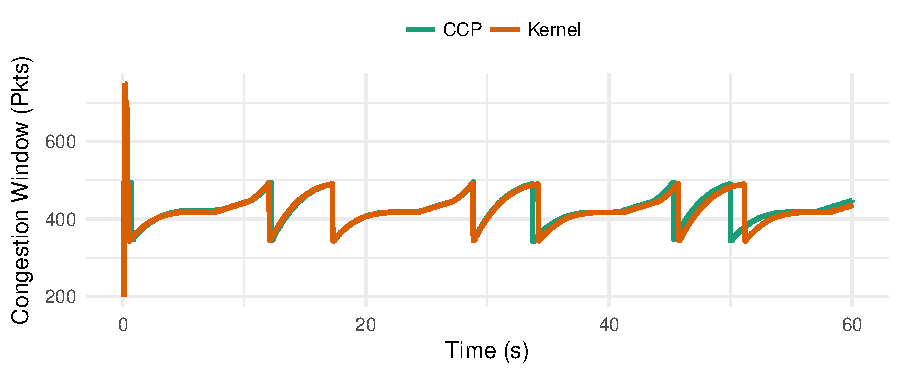
\includegraphics[width=0.95\columnwidth]{ccp/img/cubic-3-cwnd-evo-new}
    \caption{Cubic in CCP matches Cubic in Linux TCP.}\label{fig:eval:fidelity:time}
\end{figure}

\subsubsection{Throughput and Delay.}
\label{sec:eval:fidelity:tput-delay}

We study the following scenarios:

\paragrapha{Fixed-rate link (``fixed'')} A 20 ms RTT link with a fixed $96$ Mbit/s rate and 1 BDP of buffering.

\paragrapha{Cellular link (``cell'')} A 20 ms RTT variable-rate link with a 100-packet buffer based on a Verizon LTE bandwidth trace~\cite{mahimahi}.

\paragrapha{Stochastic drops (``drop'')} A 20 ms RTT link with a fixed $96$ Mbit/s rate, but with $0.01$\% stochastic loss and an unlimited buffer. To ensure that both tested algorithms encountered exactly the same conditions, we modified Mahimahi to use a fixed random seed when deciding whether to drop a packet.

These three scenarios represent a variety of environments congestion control algorithms encounter in practice, from predictable to mobile to bufferbloated paths. We calculate, per-RTT over twenty 1-minute experiments, the achieved throughput (\ref{fig:eval:fidelity:tput-cdf}) and delay (\ref{fig:eval:fidelity:delay-cdf}), and show the ensuing distributions in Figure~\ref{fig:eval:fidelity:cdfs}.

Overall, both distributions are close, suggesting that CCP's implementations make the same congestion control decisions as the kernel.

\begin{figure}
\centering
\begin{subfigure}{0.95\textwidth}
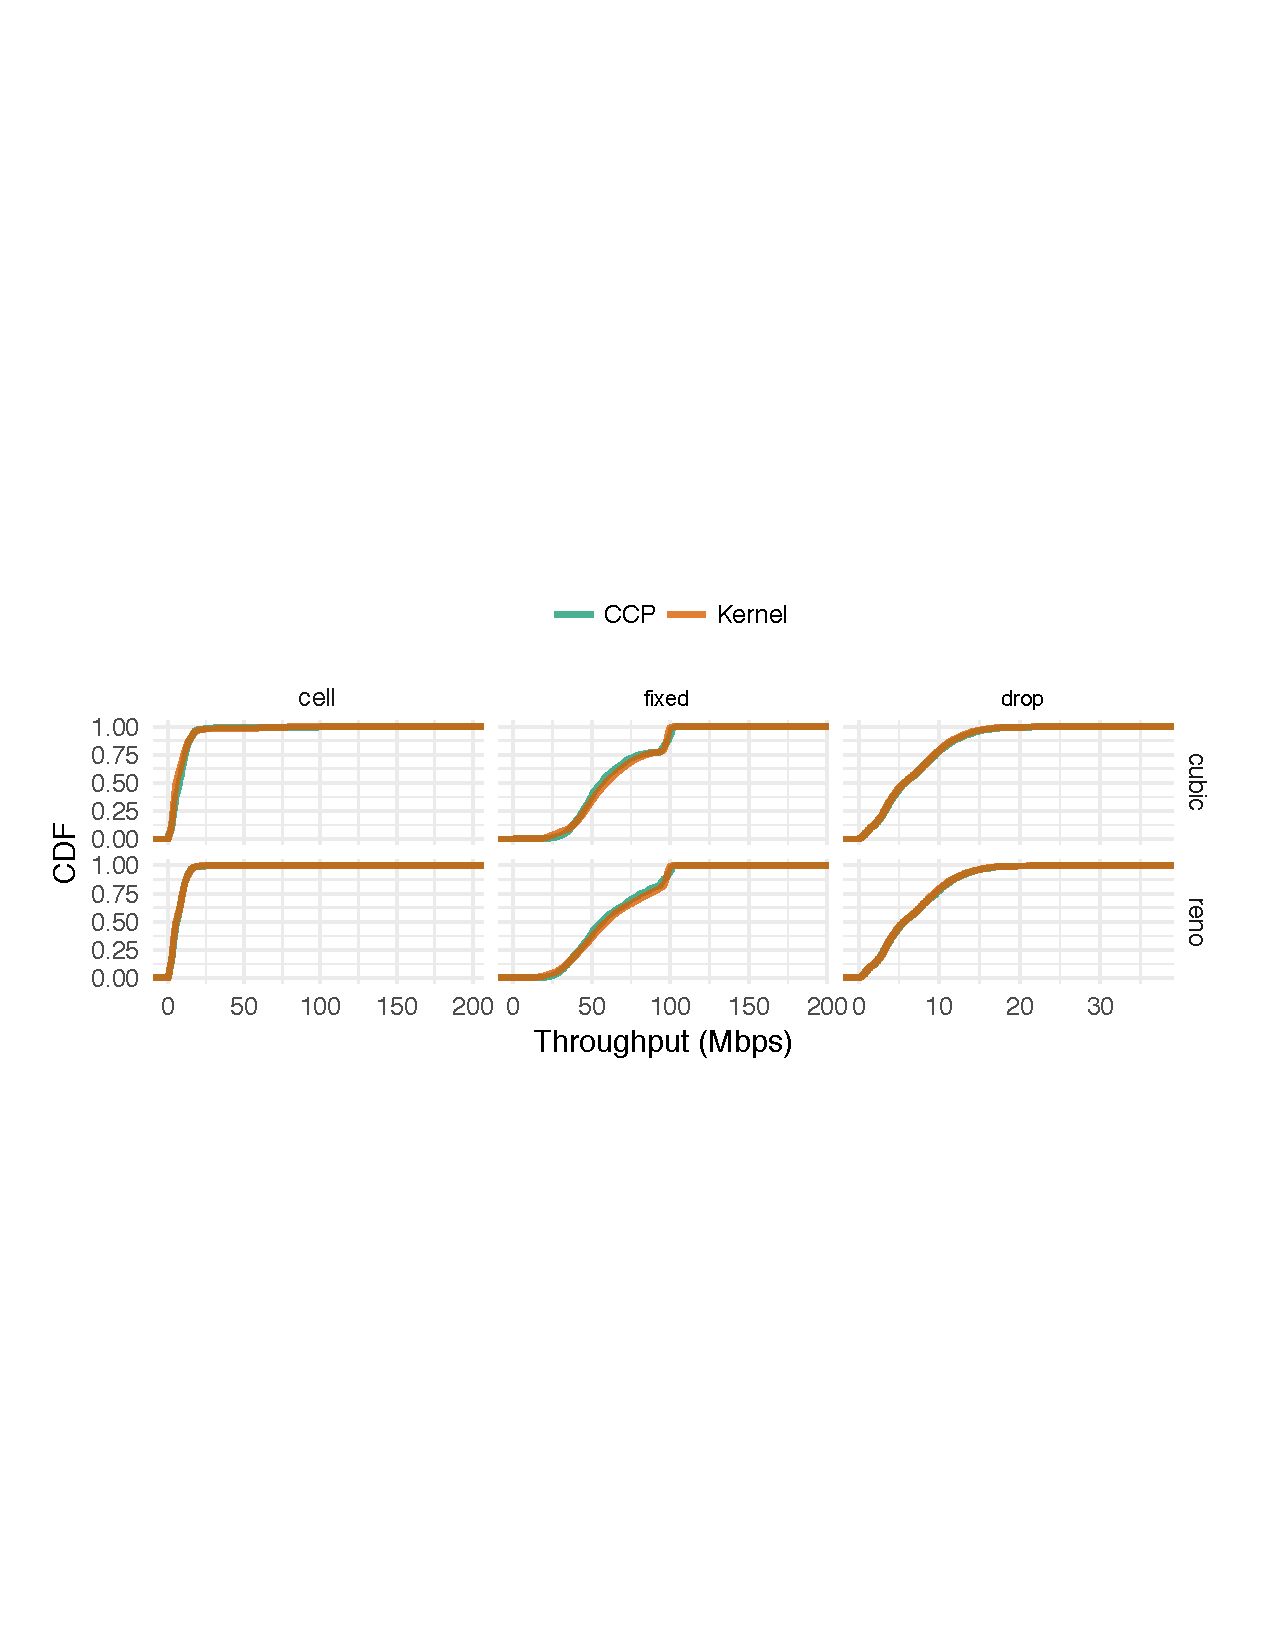
\includegraphics[width=0.95\textwidth]{ccp/img/throughput-cdf-flat}
\subcaption{Achieved throughput over 1 RTT periods. Note the different scales on the x-axes for the three scenarios.}\label{fig:eval:fidelity:tput-cdf}
\end{subfigure}
%
\begin{subfigure}{0.95\textwidth}
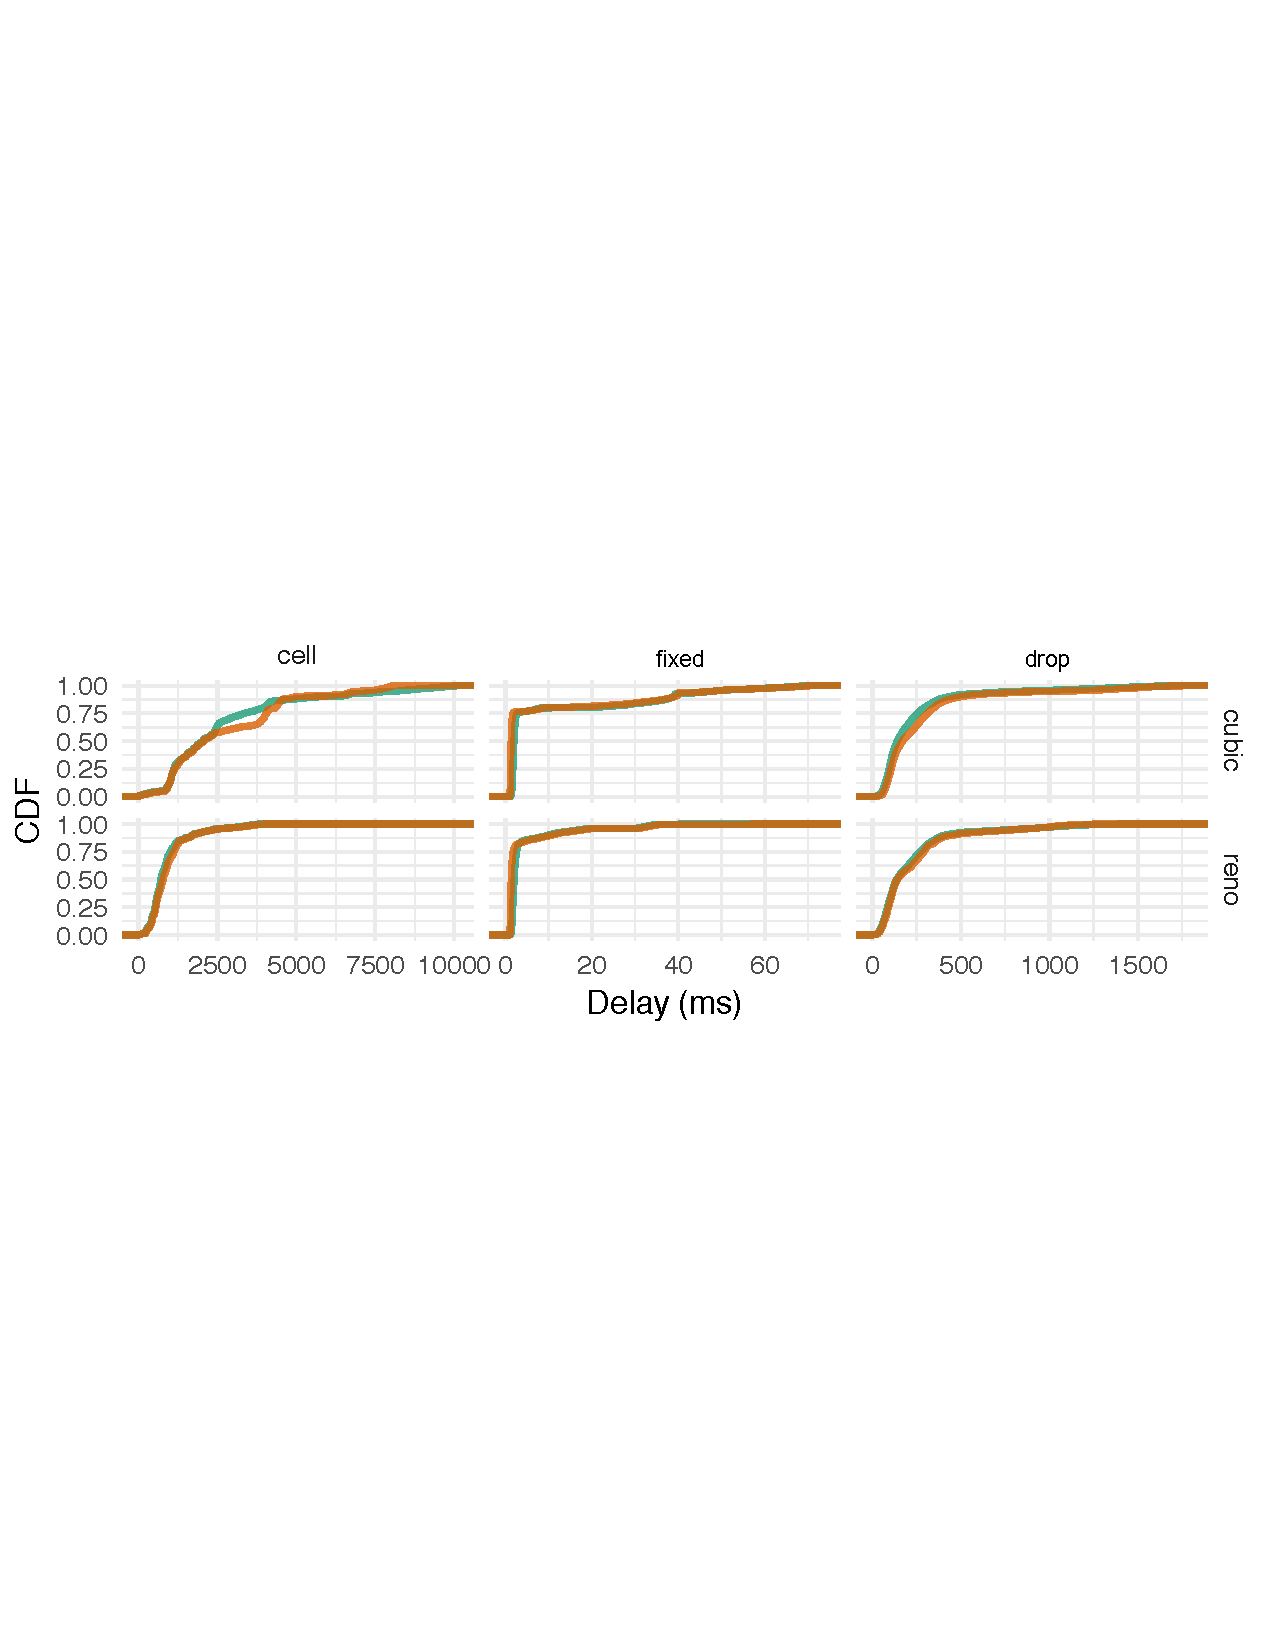
\includegraphics[width=0.95\textwidth]{ccp/img/delay-cdf-flat}
\subcaption{Achieved queueing delay over 1 RTT periods. Note the varying scales on the x-axes for the three scenarios.}\label{fig:eval:fidelity:delay-cdf}
\end{subfigure}
%
\caption{Comparison of achieved throughput over 20 ms periods. The achieved throughput distributions are nearly identical across the three scenarios and two congestion control algorithms evaluated.}\label{fig:eval:fidelity:cdfs}
\end{figure}

\subsubsection{Flow Completion Time.}
\label{sec:eval:fidelity:fct}

\begin{figure}
\centering
\begin{subfigure}{\textwidth}
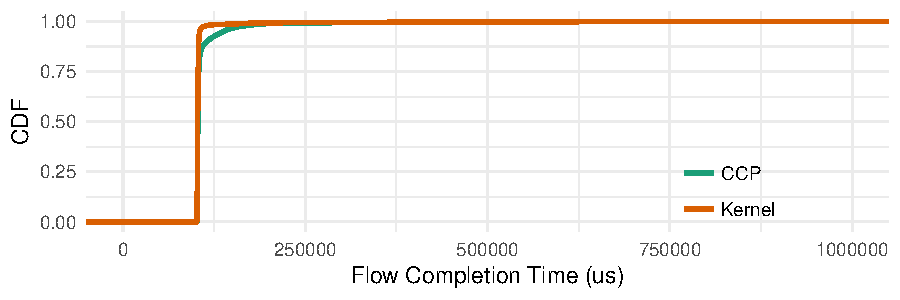
\includegraphics[width=0.95\textwidth]{ccp/img/small_fcts}
\subcaption{0-10KB Flows}\label{fig:eval:fidelity:fct:sml}
\end{subfigure}
%
\begin{subfigure}{\textwidth}
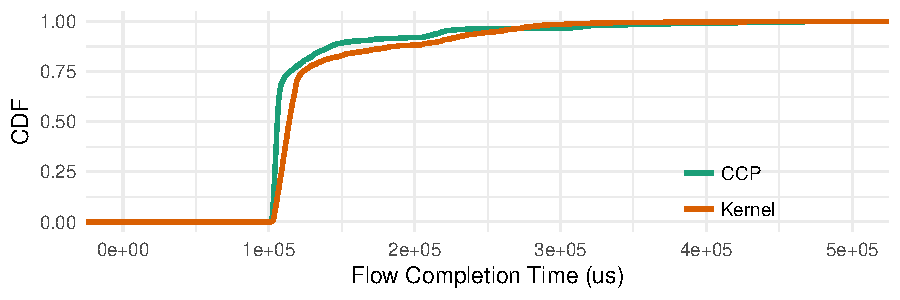
\includegraphics[width=0.95\textwidth]{ccp/img/med_fcts}
\subcaption{10KB-1MB Flows}\label{fig:eval:fidelity:fct:med}
\end{subfigure}
%
\begin{subfigure}{\textwidth}
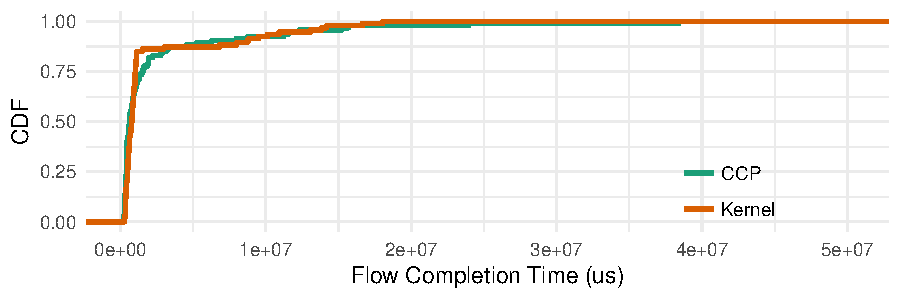
\includegraphics[width=0.95\textwidth]{ccp/img/big_fcts}
\subcaption{1MB+ Flows}\label{fig:eval:fidelity:fct:big}
\end{subfigure}
\caption{CDF comparisons of flow completion times. Note the differing x-axes.}\label{fig:eval:fidelity:fct}
\end{figure}

To measure flow completion times (FCT), we use a flow size distribution compiled from CAIDA Internet traces~\cite{caida} in a similar setting to the ``fixed'' scenario above; we use a $100$ ms RTT and a $192$ Mbit/s link.
To generate traffic, we use a traffic generator to sample flow sizes from the distribution and send flows of that size according to a Poisson  arrival process to a single client behind the emulated Mahimahi link. We generate flows with 50\% average link load, and generate $100,000$ flows to the client from $50$ sending servers using persistent connections to the client.
We used Reno as the congestion control algorithm in both cases. To ensure that the kernel-native congestion control ran under the same conditions as the CCP implementation, we disabled the slow-start-after-idle option.

Of the $100,000$ flows we sampled from the CAIDA workload, $97,606$ were $10$ KB or less, comprising $487$ MB, while the $95$ flows greater than $1$ MB in size accounted for $907$ MB out of the workload's total of $1.7$ GB.

Across all flow sizes, CCP achieves FCTs 0.02\% lower than the kernel in the median, 3\% higher in the $75^{\text{th}}$ percentile, and $30$\% higher in the $95^{\text{th}}$ percentile.

\paragrapha{Small flows} Flows less than $10$ KB in size, shown in Figure~\ref{fig:eval:fidelity:fct:sml}, are essentially unaffected by congestion control. These flows, the vast majority of flows in the system, complete before either CCP algorithms or kernel-native algorithms make any significant decisions about them.

\paragrapha{Medium flows} Flows between $10$ KB and $1$ MB in size, in Figure~\ref{fig:eval:fidelity:fct:med}  achieve $7\%$ lower FCT in the median with CCP because CCP slightly penalizes long flows due to its slightly longer update period, freeing up bandwidth for medium size flows to complete.

\paragrapha{Large flows} CCP penalizes some flows larger than $1$ MB in size compared to the native-kernel implementation: $22$\% worse in the median (Figure~\ref{fig:eval:fidelity:fct:big}).

\subsection{Performance}
\label{sec:eval:whyfold}

\subsubsection{Measurement Staleness.}
\label{sec:eval:whyfold:stale}
\begin{figure}
\centering
    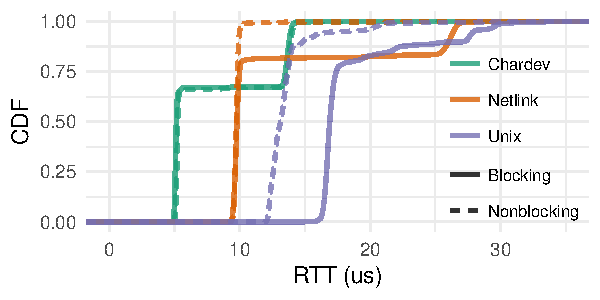
\includegraphics[width=0.95\textwidth]{ccp/img/ipc}
    \caption{Minimum time required to send information to the datapath and receive a response using different IPC mechanisms.}\label{fig:eval:ipc-latency}
\end{figure}

Because our CCP implementation, Portus, runs in a different address space than datapath code, there is some delay between the datapath gathering a report and algorithm code acting upon the report.
In the worst case, a severely delayed measurement could cause an algorithm to make an erroneous window update.

Fortunately, as Figure~\ref{fig:eval:ipc-latency} shows, this overhead is small. We calculate an IPC RTT by sending a time-stamped message to a kernel module (or \userspace{} process in the case of a Unix-domain socket). The receiver then immediately echoes the message, and we measure the elapsed time at the originating process.

We test three IPC mechanisms: Unix-domain sockets~\cite{unix-domain}, a convenient and popular IPC mechanism used for communication between \userspace{} processes; Netlink sockets~\cite{netlink}, a Linux-specific IPC socket used for communication between the kernel and \userspace{}; and a custom kernel module, which implements a message queue that can be accessed (in both \userspace{} and \kernelspace{}) via a character device.
% a custom character device, which can be read from and written to in both \userspace{} and \kernelspace{}.
%our custom kernel module, which implements a message queue that processes (or the kernel) can use via a character device.
% that processes can read from and write to.

In all cases, the $95^{\text{th}}$ percentile latency is less than $30$ $\mu$s. 

\subsubsection{Scalability.}
\label{sec:eval:whyfold:scale}

\begin{figure}
\centering
    \begin{subfigure}{\textwidth}
        \centering
        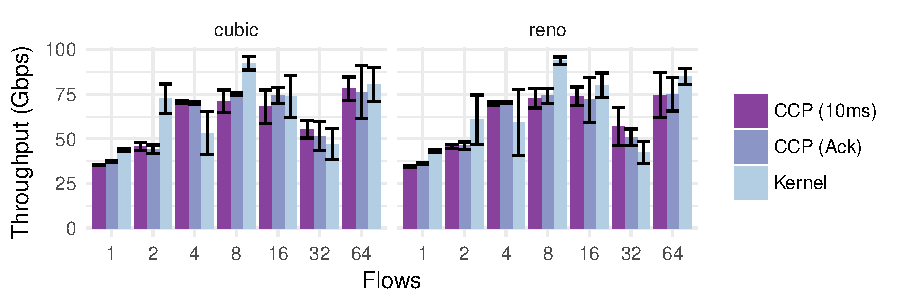
\includegraphics[width=0.95\textwidth]{ccp/img/tputs}
        \subcaption{Achieved localhost throughput as the number of flows increases}\label{fig:eval:perf:numflows}
    \end{subfigure}
    \begin{subfigure}{\textwidth}
        \centering
        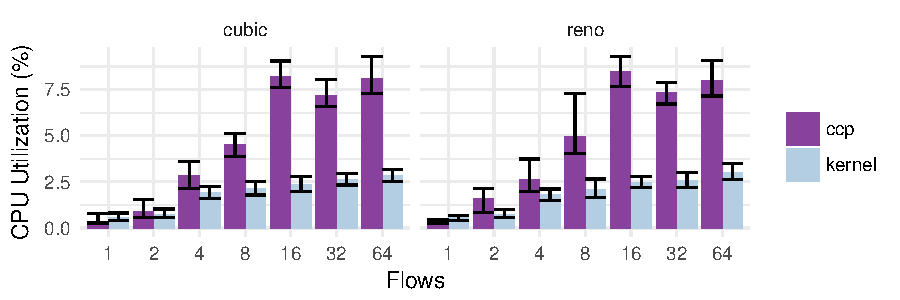
\includegraphics[width=0.95\textwidth]{ccp/img/10G_cpu_util_new}
        \subcaption{CPU Utilization when saturating a 10 Gbit/s link.}\label{fig:eval:perf:10g}
    \end{subfigure}
    \caption{CCP can handle many concurrent flows without significant CPU overhead. Error bars show standard deviation.}\label{fig:eval:perf}
\end{figure}

CCP naturally has nonzero overhead since more context switches must occur to make congestion control decisions in user-space.
We test two scenarios as the number of flows in the system increases exponentially from $1$ to $64$.
In both scenarios, we test CCP's implementation of Reno and Cubic against the Linux kernel's. We measure average throughput and CPU utilization in $1$ second intervals over the course of $10$ $30$-second experiments using iperf~\cite{iperf}. We evaluate CCP with two fold functions: one which implements a reporting interval of $10$ ms, and another which reports on every packet.

We omit mTCP and QUIC from these scalability micro-benchmarks and focus on the kernel datapath. The QUIC toy server is mainly used for integration testing and does not perform well as the number of flows increase; we confirmed this behavior with Google's QUIC team. Similarly, after discussion with the mTCP authors, we were unable to run mTCP at sufficient speeds to saturate a localhost or 10 Gbit/sec connection.

\paragrapha{Localhost microbenchmark} We measure achieved throughput on a loopback interface as the number of flows increases. As the CPU becomes fully utilized, the achieved throughput will plateau. Indeed, in Figure~\ref{fig:eval:perf:numflows}, CCP matches the kernel's throughput up to the maximum number of flows tested, 64. 
%\ma{we said that we tested up to 1024 flows at the beginning of this section. but the results are up to 64 flows?}

\paragrapha{CPU Utilization} To demonstrate the overhead of CCP in a realistic scenario, we scale the number of flows over a single $10$ Gbit/s link between two physical servers and measure the resulting CPU utilization.
Figure~\ref{fig:eval:perf:10g} shows that as the number of flows increases, the CPU utilization in the CCP case rises steadily. The difference between CCP and the kernel is most pronounced in the region between $16$ and $64$ flows, where CCP uses $2.0\times$ as much CPU than the kernel on average; the CPU utilization nevertheless remains under 8\% in all cases.

In both the CPU utilization and the throughput micro-benchmarks, the differences in CPU utilization stem from the necessarily greater number of context switches as more flows send measurements to CCP. Furthermore, the congestion control algorithm used does not affect performance.

\subsection{Low-RTT and High Bandwidth Paths}
\label{sec:eval:lowrtt}

\begin{figure}
    \centering
    \begin{subfigure}{\textwidth}
    \centering
    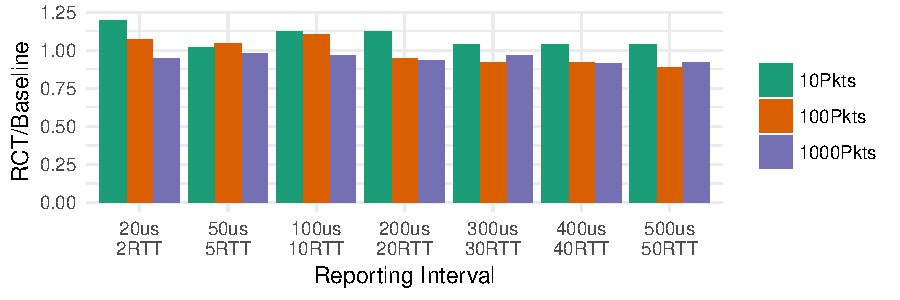
\includegraphics[width=0.95\textwidth]{ccp/img/10g-rct}
    \subcaption{Tail flow completion time at 10 Gbit/s}\label{fig:eval:lowrtt:10g}
    \end{subfigure}
    \begin{subfigure}{\textwidth}
    \centering
    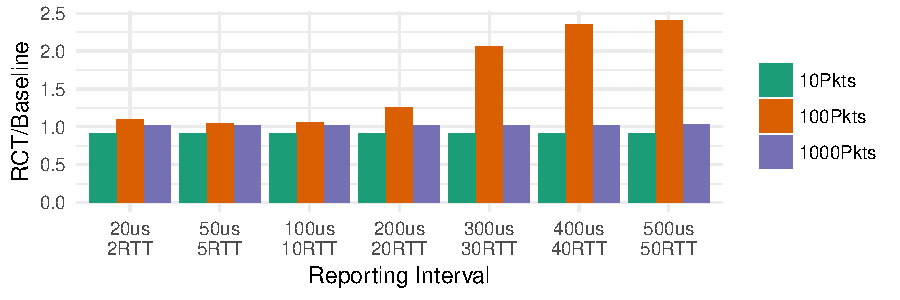
\includegraphics[width=0.95\textwidth]{ccp/img/40g-rct}
    \subcaption{Tail flow completion time at 40 Gbit/s}\label{fig:eval:lowrtt:40g}
    \end{subfigure}
    \caption{Mean tail completion across 50 simulations. While at 10 Gbit/s even rare reporting (every 50 RTTs) has limited overhead (at most 20\%), at 40 Gbit/s, a 1 ms reporting period is necessary to avoid performance degradation.}
    \label{fig:eval:lowrtt}
\end{figure}

To demonstrate it is feasible to separate congestion control from the datapath even in low-RTT and high bandwidth situations, we simulate a datacenter incast scenario using ns-2~\cite{ns2}.
We model CCP by imposing both forms of delays due to CCP: (i) the period with which actions can be taken (the reporting period) and, (ii) the staleness after which sent messages arrive in CCP. We used our microbenchmarks in \S\ref{sec:eval:whyfold:stale} to set the staleness to 20~$\mu$s, and vary the reporting interval since it is controlled by algorithm implementations. 
We used a $20$ $\mu$s RTT with a 50-to-1 incast traffic pattern across $50$ flows with link speeds of $10$ and $40$ Gbit/s. To increase the statistical significance of our results, we introduce a small random jitter to flow start times ($<$10$ \mu$s with 10 Gbit/s bandwidth and $<$2.5 $\mu$s with 40 Gbit/s bandwidth) and run each point $50$ times with a different simulator random seed value and report the mean.

Figure~\ref{fig:eval:lowrtt} compares the results with the baseline set to in-datapath window update. 
%At $10$ Gbit/s, the tail completion time is within $10$\% of that of an in-datapath update across all request sizes; at $40$ Gbit/s, the tail completion time is within $40$\% of the baseline. 
We find that at $10$ Gbit/s, CCP performance stays within $15$\% of the baseline across different flow sizes and reporting intervals ranging from $10$ $\mu$s to $500$ $\mu$s. 
Recall that $500$ $\mu$s is $50\times$ the RTT; even this infrequent reporting period yields only minor degradation.

Meanwhile, at $40$ Gbit/s the slowdown over the baseline increases with the reporting interval in the case of $100$ packet flows, but not with $10$ or $1000$ packet flows. 
Similar to the results in \S\ref{sec:eval:fidelity:fct}, the short flows and long flows are both unaffected by the reporting period because the short flows complete too quickly and the long flows spend much of their time with large congestion windows regardless of the window update.
Indeed, at $100$ $\mu$s ($10$ RTTs), the tail completion time is within $10$\% of the baseline; as the reporting increases, the tail completion time increases to over $2\times$ the baseline. 
This nevertheless suggests that when reporting intervals are kept to small multiples of the RTT, tail completion time does not suffer.
